\chapter{Command Line Interface, Terminal, and Shell}\label{ch:cli_terminal_shell}

% \begin{flushright}{\slshape
%     I am just testing some citations, \\
%     at the beginning of chapters} \\ \medskip
%     --- \textbf{Aristotle}
% \end{flushright}

% \medskip

Most User Interfaces (\acs{UI}) rely on visual cues to guide the user. For example, on Microsoft Windows, the user can use the mouse (or the finger in a touchscreen device) to click on an icon representing a folder to see its contents. Another example would be that, by clicking on a \texttt{x} symbol at the top right edge\marginnotes{In Apple and Linux systems, this symbol might be on the top left edge} of an application, the application is closed. As yet another example, drop-down menus with items such as File, Edit, and About, are commonplace, as seen in Figure \ref{fig:ch1_notepad}.
\begin{figure}[!htbp]
  \centering
        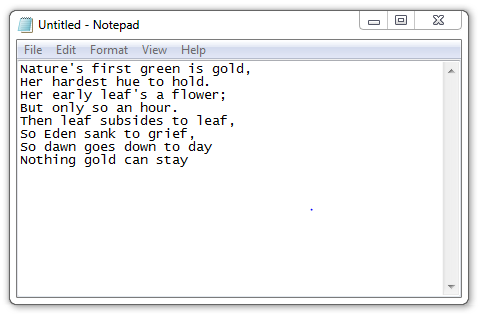
\includegraphics[width=0.85\textwidth]{Images/Chapter1/notepad.png}
        \caption{Notepad application for Windows 7.}
        \label{fig:ch1_notepad}
\end{figure}

A \acs{UI} that relies of visual cues, as the ones described above, is called a \ac{GUI}. The invention of such interfaces played a major role in the popularization of computers in the 80s. This is due to the fact that most users are more comfortable using such interfaces, as opposed to Command Line Interfaces (\acs{CLI}) that have been around since the late 60s.

In a \acs{CLI}, as opposed to an intuitive graphical interface, the user is presented with a \textbf{shell}\marginnotes{Shells are explained in Sections \ref{sec:ch1_terminology} and \ref{sec:ch1_sells}} prompt in which it can write commands to be interpreted by the \textbf{shell}. You can see an example below of a \acs{CLI} in which a user entered the command \textbf{\texttt{ls}} to list all files and folders in the working directory\marginnotes{In this book, the words \textbf{folder} and \textbf{directory} are used interchengeably}.

\begin{command_line}[Bash]
marcel@dell:~$ ls
Documents      Downloads      Pictures
Music          Video          seneca.pdf
marcel@dell:~$
\end{command_line}

In order to properly use a \acs{CLI}, the user needs to learn a series of commands that the shell understands, as well as the syntax of these commands. Hence, it should come to no surprise that most regular users prefer to use \acs{GUI}s which do not incur in such steep learning curves.

If you are reading this book, however, I expect you not to be a regular user. In fact, I expect you to be starting a career as systems analyst, a software developer, or other positions in the IT industry. For people like you, having a clear understanding of how to use a \acs{CLI} presents a number of advantages:
\begin{itemize}
    \item There are tasks that can only be achieved by using a \acs{CLI} because no \acs{GUI} has been created to perform them.
    \item Some tasks can be performed, using a \acs{CLI}, in a fraction of the time it would take using a \acs{GUI} tool.
    \item \acs{CLI}s can be accessed remotely in a fast and straightforward fashion, allowing you to control multiple systems from a single computer
    \item Users can quickly create scripts that run on \acs{CLI}s to automate repetitive tasks such as: adding new users to the system, backing up data, updating the system, etc.
    \item The steps required to perform some actions using \acs{GUI}s can vary a lot depending on which \acs{OS}, or Linux distribution, you are using. On the other hand, they are normally identical using a CLI. In fact, the same commands\marginnotes{With a few notable exceptions} can be used in all Linux distributions, Apple computers, and since 2016, even in Windows systems.
\end{itemize}

Most Linux distributions have a \acs{GUI} that allow regular users to achieve daily tasks such as web browsing, email, or writing documents. However, all Linux distributions also come with a terminal emulator that allow super users to do much more using a \acs{CLI}.

\section{Terminology}
\label{sec:ch1_terminology}

Before moving forward to learn how to use a Linux \acs{CLI}, It is important to notice the difference between three concepts that are often used interchangeably:

\begin{description}
\item[CLI] The \acs{CLI} is just the technical name of the method by which we interact with a computer by means of written instructions.
\item[Terminal] All major Linux distributions have a \acs{GUI}. However, they normally also provide you with a terminal, or more precisely a terminal emulator. A terminal emulator is nothing else than a program that provides us with a \acs{CLI} to interact with the \textbf{shell}.
\item[Shell] The \textbf{shell} is a software that reads keyboard commands and passes them to the \acs{OS} to carry out. Such commands could be used to perform simple tasks like listing the files in a particular folder, adding users to the system, creating folders, or complex tasks such as upgrading the \acs{OS}, installing applications, etc.
\end{description}


\section{Shells}
\label{sec:ch1_sells}

As mentioned before, a \textbf{shell} is a software that interprets commands passed by the user, and passes them to the \acs{OS}. However, just like there are multiple languages such as English, Spanish, or Mandarim, there are multiple shells available. Table~\ref{tab:ch1_shells} below presents a description of a few such shells\marginnotes{Many other shells exist, such as dash, ksh, etc}.

\begin{table}[!htbp]
   \myfloatalign
   \begin{tabularx}{\textwidth}{Xp{90mm}} \toprule
   %\tableheadline{Shell} & \tableheadline{Description}\\ \midrule
   \textbf{sh} & The Bourne shell, which has been distributed as the default \textbf{shell} for Unix since 1979. \\
   \textbf{bash} & Bourne Again Shell, an upgraded version of \textbf{sh}, written by the GNU Project, which has become the \textit{de facto} standard Linux shell. \\
   \textbf{csh} or \textbf{tcsh} & A Unix shell using a syntax similar to the \textbf{C} programming language. \textbf{tcsh} is identical to \textbf{csh}, with the addition of some extra features such as command-line completion.\\
   \bottomrule
   \end{tabularx}
\caption{List of Linux Shells.}
\label{tab:ch1_shells}
\end{table}

In this book, we will cover exclusively the \textbf{bash shell}. This is due to the fact that \textbf{bash} is the default shell for the most widely used Linux distributions. In fact, it is hard to find a Linux distribution that does no come with a \textbf{bash shell}. That said, after learning how to use one shell, it is much easier to learn other shells, as they share many concepts and syntax.

\section*{Exercises}
\addcontentsline{toc}{section}{Exercises}

\begin{exercises}
   \item Explain, with your own words, what is a Command Line Interface (\acs{CLI}).
   \item Explain, with your own words, what is a Graphical User Interface (\acs{GUI}).
   \item What is the relationship between a terminal emulator, and a shell?
   \item Which commands are used to list all files in the working directory using the following shells: sh, bash, csh, dash, and ksh?
\end{exercises}
